\section{HEAVY-FLAVOR PRODUCTION}
\label{heavyflavor}
Charm and beauty production provides a well calibrated probe for experimental investigation of heavy-ion collisions. The initial heavy-quark distributions are calculable from perturbative QCD and the calculations can be verified with pp measurements. However, the large advantage is that this probe is conserved from its production at early stage of the collision until it escapes from interaction region, and is eventually detected. This means that it is well tagged, which opens a possibility of a direct access to its interactions in the QGP, including the low- and intermediate-$p_{\rm T}$ regime. Two observables are usually studied: the nuclear modification factor $R_{\rm AA}$, and azimuthal-flow anisotropy, measured as the elliptic-flow coefficient $v_2$. They are closely connected: the in-medium heavy-quark energy loss decreases the momenta of heavy quarks, they may then thermalize in the surrounding matter, and thus participate in the evolution of collective-flow. The simultaneous measurement of the $R_{\rm AA}$ and $v_2$ enables the determination of the heavy-flavour transport coefficients.


Detection of heavy-flavor particles are done by two methods. The primary tool is invariant-mass reconstruction of exclusive particle decays in a secondary vertex, displaced from the interaction one. In the second method the heavy-flavor spectra are inferred from the lepton ($\mu^\pm$ or e$^\pm$) $p_{\rm T}$ spectra, presuming that these leptons are produced in semi-leptonic decays of heavy-flavor particles. However, this way a $p_{\rm T}$-dependent mixture of charm and beauty hadrons is measured. When possible, a requirement that the lepton is not coming from the interaction vertex is utilized, which significantly suppresses the background, especially at lower $p_{\rm T}$ (below 4~GeV). The B-meson production is also accessible with the inclusive decays ${\rm B} \rightarrow {\rm J}/\psi + X$, demanding the J/$\psi$ decay vertex to be separated from the interaction point.

\subsection{Heavy-Flavor Spectra}
\label{subsecks:heavyspectra}
The $p_{\rm T}$ spectra of heavy-flavour particles are measured by ALICE in pp, Pb--Pb, and p--Pb collisions. The pp results are compared to perturbative QCD calculations and other models~\cite{ALICE:2011aa,Abelev:2012vra}, giving information about preferred values for parameters, such as renormalization and factorization scales. The charm-particle spectra are measured down to very low $p_{\rm T}$ (about 1~GeV in pp) allowing for precise determination of the total charm cross section at LHC energies. The pp spectra also serve as a normalization for Pb--Pb measurements~\cite{ALICE:2012ab}.

The heavy-flavor spectra in heavy-ion collisions are expected to be suppressed with respect to those in pp interactions, due to the energy loss of heavy quark when traversing the dense medium. However, the energy loss of heavy quarks is predicted to be different than that of light quarks and gluons. Energy loss of quarks by bremsstrahlung radiation will be quark-mass dependent. Due to a destructive interference, such gluon radiation is suppressed in directions close to that of the initial quark, for angles smaller than $\Theta_0 \approx m/E = 1/\gamma$ ($m$, $E$, and $\gamma$ being the quark mass, energy, and gamma-factor, respectively). For a given momentum, this exclusion region (i.e. $\Theta_0$) is larger for the heavier quarks, resulting in smaller energy loss for heavy quarks compared to that for the light ones. This so called dead-cone effect was originally described for the QCD radiation in vacuum~\cite{Dokshitzer:1991fc}, and later applied to the medium-induced radiation in a similar manner~\cite{Dokshitzer:2001zm}. The predicted mass hierarchy is stronger at $p_{\rm T}$ comparable with quark masses, and diminished progressively at higher $p_{\rm T}$. Recent model calculations include both the radiation and collisional energy losses, which increases the suppression of heavy quarks, and leading to \Raa\ values closer to the expectation for light quarks.

 Additional effects that can modify the expected suppression pattern have also to be taken into account. Contrary to heavy-flavor hadrons, produced by fragmentation of the corresponding heavy quarks, light-flavor particles at $p_{\rm T} \sim {\cal O}(10)$~GeV are, at the LHC energies, mostly produced in gluon fragmentation. However, gluons have by a factor 9/4 larger color charge than quarks, and consequently a gluon is expected to loose more energy than a quark. This color-charge effect is increasing the expected difference in suppression between the light- and heavy-flavor particles. Other effects of less importance are taken into account in various models, such as nuclear modification of structure functions and harder fragmentation function for heavy quarks compared to the light ones.

Charm mesons are identified reconstructing the following decays: ${\rm D}^0 \rightarrow {\rm K}^-\pi^+$, ${\rm D}^+ \rightarrow {\rm K}^-\pi^+\pi^+$, and ${\rm D}^{*+} \rightarrow {\rm D}^0\pi^+$ (and their antiparticles), requiring the decay vertex of ${\rm D}^0$ and ${\rm D}^+$ to be displaced from the interaction point. The D-meson yields are corrected for feed-down from beauty decays, based on simulations. The B-decay contribution amounts to 5--15\,\% of the yields, depending on $p_{\rm T}$ and the particle type. The nuclear modification factor $R_{\rm AA}$ is calculated from the $p_{\rm T}$ spectra measured in both pp~\cite{ALICE:2011aa,Abelev:2012vra} and Pb--Pb~\cite{ALICE:2012ab} collisions.

 As expected, $p_{\rm T}$ dependencies of \Raa\ for three D-mesons are compatible. Therefore, an average D-meson $R_{\rm AA}$ is calculated combining the results according their uncertainties (the average is thus dominated by the ${\rm D}^0$ result). The average D-meson $R_{\rm AA}$ in central Pb--Pb collisions as a function of $p_{\rm T}$ is compared with that of charged particles in Fig.~\ref{figks:DmesonRAA}. The D-meson $R_{\rm AA}$ might be slightly above the charged-particle one, hinting at less charm-quark suppression, but the difference, if any, is very small. This tendency was recently confirmed with higher statistics charm measurements. The model calculations overlayed on data in Fig.~\ref{figks:DmesonRAA} are (I)~\cite{Sharma:2009hn,He:2011pd}, (II)~\cite{Horowitz:2011cv}, (III)~\cite{Horowitz:2011wm}, (IV)~\cite{Alberico:2011zy,Monteno:2011gq}, (V)~\cite{Gossiaux:2009mk,Gossiaux:2010yx}, (VI)~\cite{Fochler:2011en}, (VII)~\cite{Buzzatti:2011vt}, and (VIII)~\cite{Armesto:2005iq}. Varying degrees of agreement with the charm results are shown by various models. In general the inclusion of collisional energy loss improves the model description. In model (I) the larger D suppression is obtained by introducing in-medium dissociation of D mesons, in addition to radiative energy loss. The remaining models that compute also the charged-particle $R_{\rm AA}$, have not reached good description for both cases, albeit some being not far.

\begin{figure}
\centering
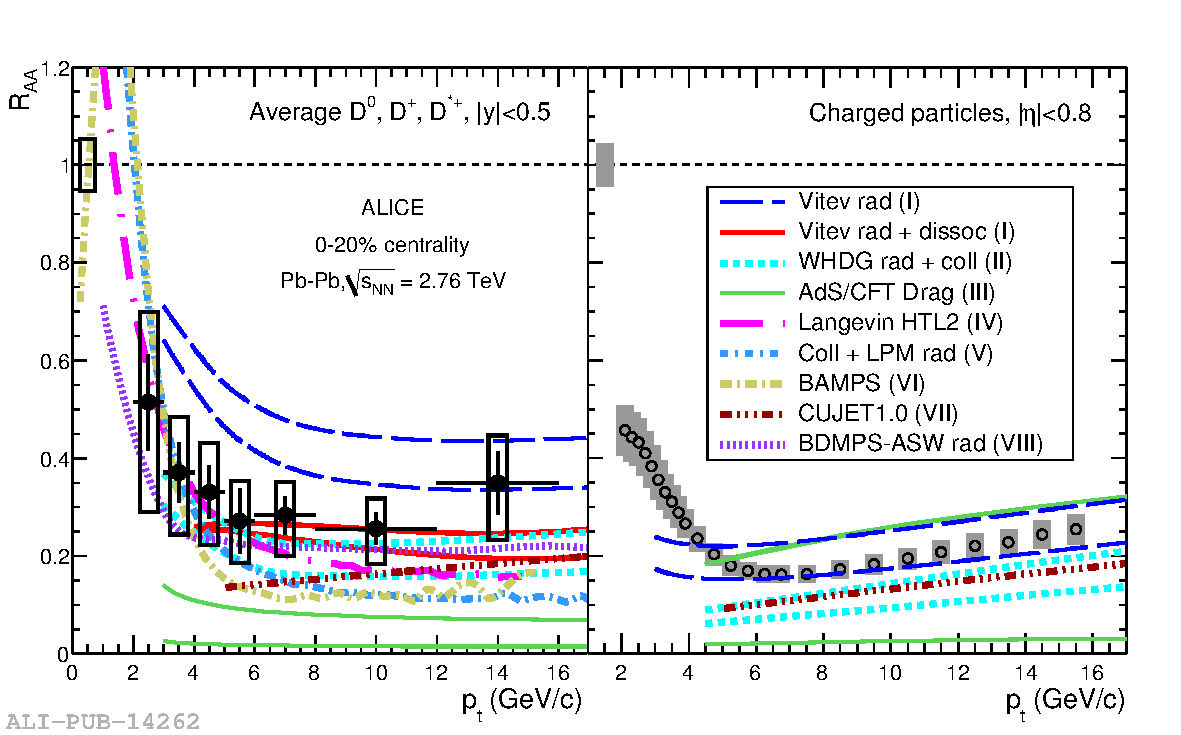
\includegraphics[width=0.7\textwidth]{heavyflavorfigs/DmesonChargedRAAmodels.pdf}
\caption{Average D-meson $R_{\rm AA}$ (left) and charged particle $R_{\rm AA}$ (right) as a function of $p_{\rm T}$ for the centrality between 0--20\,\%. The normalization uncertainties shown at unity in abscissa are almost fully correlated. The curves represent various model calculations, referred in the text, some of them are shown as a range. Reproduced from~\cite{ALICE:2012ab}.}
\label{figks:DmesonRAA}
\end{figure}

The family of measured D mesons was enlarged recently with the study of the ${\rm D}_{\rm s}^+ \rightarrow {\rm K}^+{\rm K}^-\pi^+$ decay~\cite{Abelev:2012tca}. The presence of the strange quark may lead to a relative increase of ${\rm D}_{\rm s}$ production with respect to other D-mesons, as a consequence of the general strangeness enhancement observed in heavy-ion collisions. Preliminary results show a ${\rm D}_{\rm s}$ $R_{\rm AA}$ in the $p_{\rm T}$ region 4--12~GeV larger than the D-meson $R_{\rm AA}$, however, still within large uncertainties.

The behavior of the charm-meson $R_{\rm AA}$ has been confirmed by the ALICE measurement of the muon spectrum in the forward region $2.5 < y < 4$~\cite{Abelev:2012qh}. The estimated pion- and kaon-decay contribution is subtracted from the measured muon spectrum, this contamination is below 10\,\% for $p_{\rm T} > 4$~GeV, where the results are presented. The corrected muon $p_{\rm T}$ spectrum thus represents the result for a mixture of muons from semi-leptonic charm and beauty decays, presumably charm dominated at $p_{\rm T}$ about 4~GeV and progressively becoming beauty dominated for $p_{\rm T} > 6$~GeV. The heavy-flavor muon $R_{\rm AA}$, using an analogous analysis of pp data for normalization, is presented in Fig.~\ref{figks:HFmuonRAA}. The muon $p_{\rm T}$, being correlated with the heavy-flavor-particle $p_{\rm T}$, is systematically smaller than the latter (for $p_{\rm T}$ above a few GeV). The comparison with the D-meson $R_{\rm AA}$ shows qualitative agreement, since the $p_{\rm T}$ dependence is rather flat. A similar measurement exploiting electron detection in the mid-rapidity region has been also reported~\cite{Abelev:2012xe}.

\begin{figure}
\centering
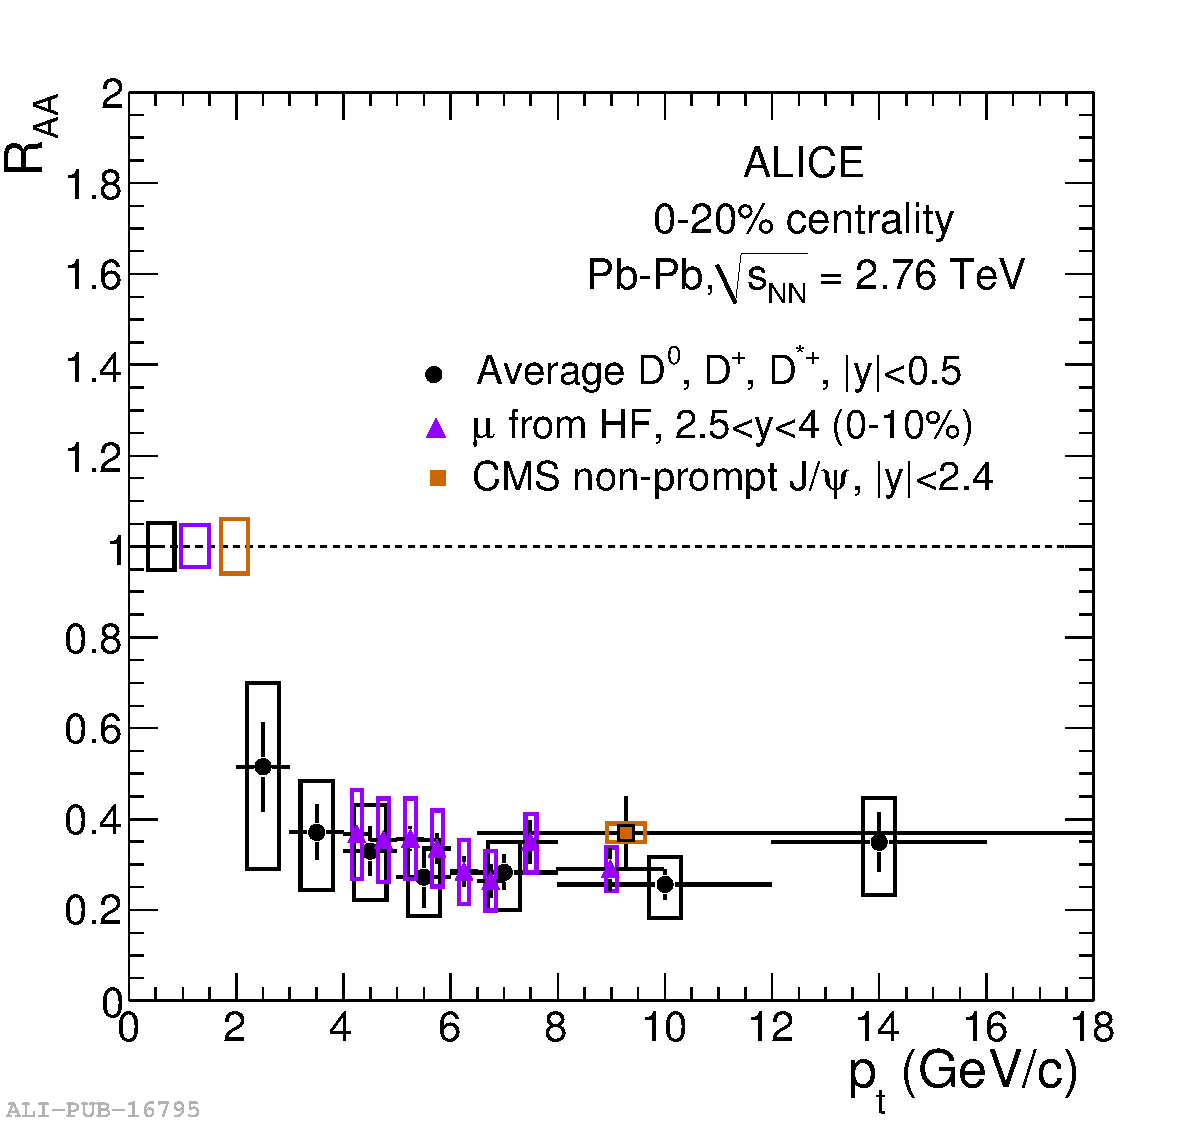
\includegraphics[width=0.5\textwidth]{heavyflavorfigs/DmesonHFmuonBRAA.pdf}
\caption{Heavy-flavor muon $R_{\rm AA}$ as a function of $p_{\rm T}$ compared to the average D-meson $R_{\rm AA}$. Results are for 0--20\,\% centrality class of Pb--Pb collisions. CMS preliminary result for beauty $R_{\rm AA}$ from measurement of non-prompt J/$\psi$ is shown with square. Reproduced from~\cite{Abelev:2012qh}.}
\label{figks:HFmuonRAA}
\end{figure}

The preliminary CMS result for $R_{\rm AA}$ from the measurement of non-prompt J/$\psi$ is also shown~\cite{Chatrchyan:2012np} in Fig.~\ref{figks:HFmuonRAA}. The position of the J/$\psi$-decay point with respect to interaction vertex is used to select non-prompt J/$\psi$ particles, practically exclusively originating from B-meson decays. Higher-statistics results on the centrality dependence of the $R_{\rm AA}$ for non-prompt J/$\psi$~\cite{CMS:2012wba} (in $p_{\rm T}$ range 6.5--30~GeV) compared to the ALICE D-meson data (in $p_{\rm T}$ range 8--16~GeV) indicate smaller suppression for beauty production than for charm production, except for peripheral collisions, where the measurements are within the respective uncertainties. The difference in the used $p_{\rm T}$ ranges takes into account that the J/$\psi$ momentum is decreased in the decay with respect to B-meson one. For the first time the predicted hierarchy of the charm and beauty energy loss is experimentally confirmed.

\subsection{Charm Elliptic Flow}
\label{subsecks:heavyflow}
 An elliptic azimuthal asymmetry is caused by the asymmetric collision geometry: in semi-central collisions the overlapping region of the two colliding nuclei has an almond shape, elongated in the direction perpendicular to the event plane (the plane defined by the beam axis and the centers of the two nuclei). This initial space asymmetry is transferred by the pressure created in the medium into an asymmetry in the azimuthal momentum distribution, resulting in more final particles produced in the event plane than out of the event plane. The azimuthal distribution is described by $\propto 1 + v_2 \cos{2(\varphi - \psi)}$, where $\varphi - \psi$ is the particle azimuthal angle with respect to the event-plane (at azimuthal angle $\psi$), and the coefficient $v_2$ characterizes the amplitude of the azimuthal modulation. The position of the event plane $\psi$ is estimated with a set of the particle tracks in the same event.

The elliptic flow of charm has been studied by ALICE for the three mesons: ${\rm D}^0$, ${\rm D}^+$, and ${\rm D}^{*+}$, and, since the $v_2$ values are compatible, they are then averaged applying beforehand the feed-down correction like in the case of the D-meson $R_{\rm AA}$. The $v_2$ results for the average D meson are presented in Fig.~\ref{figks:DmesonV2} for the centrality range 30--50\,\%. The comparison with the charged-particle $v_2$ obtained with the same method reveals that the $v_2$ values for $p_{\rm T}$ between 2--8~GeV are compatible. This is the first direct observation of non-zero $v_2$ for a heavy-flavor particle. The large value of the charm $v_2$ at $p_{\rm T}$ around 2~GeV is interpreted as a signature of the in-medium thermalization of charm quarks. The challenge now is a simultaneous model description of the charm \Raa\ and $v_2$ measurements. This needs detailed transport model calculations, since the results are sensitive to the time evolution of the suppression and the elliptic-flow build-up.

\begin{figure}
\centering
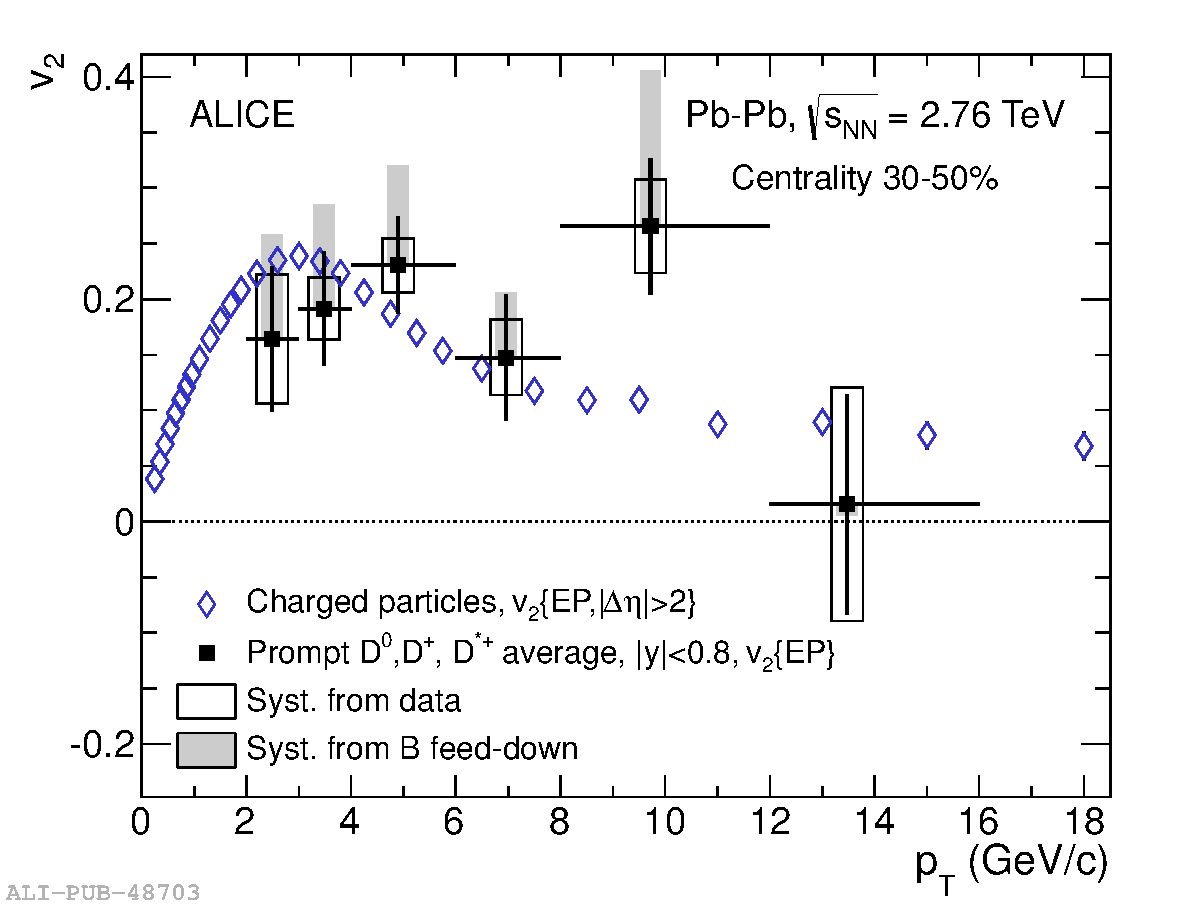
\includegraphics[width=0.5\textwidth]{heavyflavorfigs/DmesonV2.pdf}
\caption{Elliptic-flow coefficient $v_2$ obtained with the event-plane method, as a function of $p_{\rm T}$ for the centrality 30--50\,\%, averaged for ${\rm D}^0$, ${\rm D}^+$, and ${\rm D}^{*+}$, compared to the charged-particle measurement. Reproduced from~\cite{Abelev:2013lca}.}
\label{figks:DmesonV2}
\end{figure}

At higher $p_{\rm T}$ a positive $v_2$ can be generated by the difference in the in-medium path lengths for charm quarks emitted in-plane compared to those emitted out-of-plane. The shorter path length for the in-plane partons implies less suppression, i.e. larger $R_{\rm AA}$ for particles produced in this direction, than for those produced in the out-of-plane direction. In fact, the results can be presented as an azimuthally-dependent $R_{\rm AA}$, or equivalently, as the azimuthally-integrated $R_{\rm AA}$ and the $v_2$. The interpretation of the high-$p_{\rm T}$ $v_2$ as a path-length effect opens the possibility of studying  the in-medium path-length dependence of the parton energy loss.

The $v_2$ results for D mesons are complemented by the recently reported elliptic-flow measurements at forward rapidities ($2.5 < y < 4$) for the muons from heavy-flavour decays. They show an effect of similar magnitude. Indication of non-zero heavy-flavour $v_2$ using the semi-leptonic decays were previously published by RHIC experiments~\cite{Adler:2005ab,Adare:2006nq}. 